\chapter{Algoritmo Genético}

El Algoritmo Genético (AG) es un método de computación evolutiva o \textit{machine learning}, basado en la teoría sintética de la evolución. Dicha teoría, a grandes rasgos, combina el mecanismo de la selección natural de Darwin con la genética de Mendel. Nos indica que el individuo más apto sobrevive, por lo que entre mejores sean los padres, mejor es la descendencia.

Actualmente el AG se utiliza para resolver problemas de búsqueda y optimización. Las áreas de aplicación son por ejemplo: economía, finanzas, medicina, ciencias sociales, investigación de operaciones, hidráulica, aeronáutica y química. Algunos ejemplos dentro de estas áreas son: diseño de redes de agua potable, optimización de portafolios de inversión, el problema del agente viajero y asignar asientos en un evento.

Los pasos del AG son los siguientes:

\begin{enumerate}
\item Selección: Se define una población de tamaño $n$. El valor de aptitud o adaptabilidad, de cada elemento en la población, se asigna al evaluar su utilidad en la función objetivo. Entre mejor sea el elemento, más alto será su valor de adaptabilidad. Se eligen 2 elementos de la población, llamados padres. La selección de los padres depende de qué tan aptos sean. Con dichos padres se va a formar un hijo.

\item Cruce: Con cierta probabilidad se toma información de los padres. Dicha información la llamaremos genes.

\item Mutación: Cada gen agregado al hijo tiene una probabilidad pequeña de mutar.

\item Reemplazamiento: Se repiten los 3 pasos anteriores hasta formar $n$ hijos y poder reemplazar la población.
\end{enumerate}

Con este proceso se obtiene una generación. El número de generaciones así como el tamaño de la población se fijan antes de iniciar con el algoritmo. En la \figurename{~\ref{fig_AG}} podemos ver el diagrama de los pasos mencionados.

\begin{figure}[H]
\centering
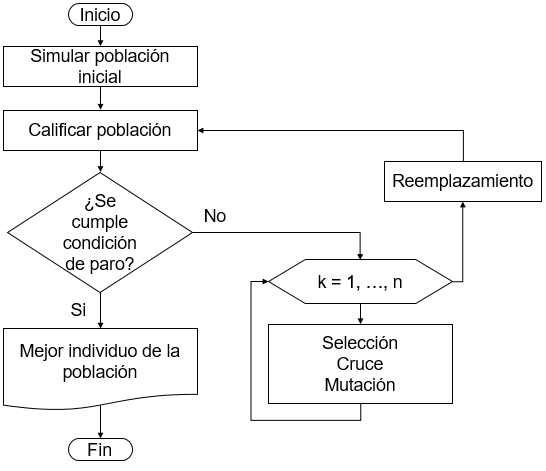
\includegraphics[scale = 0.8]{diagrama_flujo_AG} %width=\textwidth
\caption[\textit{Diagrama de flujo del Algoritmo Genético}]{\textit{Se muestra el diagrama de flujo que se sigue en el Algoritmo Genético.}}\label{fig_AG}
\end{figure}

En la siguiente sección explicaremos cómo encontramos una buena asignación utilizando el AG. Cabe mencionar que Reeves y Rowe en su libro \textit{Genetic Algorithms: Principles and Perspectives} [\ref{ReevesRowe}], nos indican que se puede generar una nueva población haciendo el cruce y la mutación o utilizando sólo una de ellas. En nuestro caso, la estrategia que seguimos fue utilizar ambas.


\section{Algoritmo Genético aplicado a los horarios}

El objetivo principal de este proyecto es obtener una matriz con la asignación final de materias, profesores y horas. Para ello haremos uso del AG. A continuación vamos a definir los términos que utilizaremos:

\begin{itemize}
\item[-] Asignación: Matriz de 3 columnas con la información de materias, profesores y horarios.

\item[-] Población: Conjunto de $n$ asignaciones.

\item[-] Padre: Asignación seleccionada, de la población, para formar un hijo.

\item[-] Gen: Vector de 3 entradas (Materia, Profesor, Horario) con la información extraída de una asignación.

\item[-] Hijo: Asignación formada a partir de los genes de 2 padres.

\item[-] Probabilidad de mutación: Debe de ser un valor pequeño. %Definimos \textit{prob\_mutacion} $ = \dfrac{1}{24} \approx 0.04$

\item[-] Generación: Se tiene una generación cuando se han creado $n$  hijos y se puede reemplazar la población.
\end{itemize}

Los pasos que seguimos para obtener la asignación final son:

\begin{enumerate}
\setcounter{enumi}{-1}
\item \textbf{Crear un archivo \textit{xlsx}} \label{paso_cero}

Crear un archivo \textit{xlsx} con 3 hojas:

\begin{itemize}
\item[-] Horario: Contiene una asignación predefinida con los grupos que se desean tener en la asignación final.

\item[-] Materias: Contiene el nombre de las materias del vector \textit{vec\_nom\_materias} (ver Sección \ref{Sec_NomMaterias}).

\item[-] Profesores: Contiene la matriz \textit{mat\_nom\_prof}, con la información de cada profesor (ver Sección \ref{nomProfesores}).
\end{itemize}

Las hojas \textit{Materias} y \textit{Profesores} nos sirven de guía para llenar de manera adecuada la hoja \textit{Horario}. Evitando los problemas vistos en las secciones mencionadas de falta de acentos, nombres incompletos, entre otros.


\item \textbf{Definir parámetros iniciales}

\begin{itemize}
\item[-] $n \in \mathbb{N}$, tamaño de la población.

\item[-] $num\_generacion \in \mathbb{N}$, número de generaciones.

\item[-] $num\_max\_asig \in \mathbb{N}$, número máximo de materias que se le pueden asignar a un profesor.

\item[-] $prob\_mutar \in (0,0.05]$, probabilidad de mutación.
\end{itemize}

\item \textbf{Fijar semilla}

Con el comando \verb@set.seed(42)@ de \textit{R}, se fija la semilla para poder replicar las simulaciones. En este caso elegimos el 42.

\item \textbf{Simular esqueleto} \label{paso_sim_esq}

Obtener la matriz \textit{mat\_esqueleto} con el procedimiento visto en la Sección \ref{sec_esqueletos}.

\item \textbf{Simular solicitudes pseudo-reales} \label{paso_sim_solicitudes}

Obtener la matriz \textit{mat\_solicitudes} con el procedimiento visto en la Sección \ref{SimSolicitudesProfesores}.


\item \textbf{Leer archivo de excel}

Con la función \verb@read_excel()@, en \textit{R}, leer la hoja \textit{Horario} del archivo creado en el paso \ref{paso_cero}.

\item \textbf{Ajustar infomación en matrices}

Eliminar la información de las solicitudes correspondiente a la asignación predefinida. Se eliminan los grupos a esa hora o con esa materia.

Eliminar los grupos de la asignación predefinida en \textit{mat\_esqueleto}.


\item \textbf{Definir matrices auxiliares}

Estas matrices nos ayudan durante el proceso sin alterar las matrices originales.

Definir \textit{mat\_aux\_esqueleto} igual a \textit{mat\_esqueleto}.

Definir \textit{mat\_aux\_solicitudes} igual a \textit{mat\_solicitudes}.

%Estas matrices nos ayudan a eliminar información que ya no necesitamos durante el proceso sin alterar las matrices originales.


\item \textbf{Generar una población inicial}

Se generan $n$ asignaciones a partir del esqueleto simulado en el paso \ref{paso_sim_esq} y de las solicitudes pseudo-reales simuladas en el paso \ref{paso_sim_solicitudes}.

Para cada asignación, comparamos el número de solicitudes con el número de grupos simulados en el esqueleto. Ésto por materia y por hora. Se tienen dos casos:

\begin{enumerate}
\item[a)] El número de solicitudes es mayor al número de grupos simulados. En este caso se asignan los grupos tomados de una muestra aleatoria de las solicitudes. El tamaño de la muestra es igual al número de grupos simulados para la materia y hora correspondientes.

\item[b)] El número de solicitudes es menor o igual al número de grupos simulados. Se asignan todos los grupos en la solicitud, para la materia y hora correspondientes.
\end{enumerate}

De esta manera se asignan todos los posibles grupos que se hayan solicitado. Se debe de considerar lo siguiente:

\begin{itemize}
\item[-] Un profesor no puede impartir diferentes materias a la misma hora.

\item[-] Un profesor no puede impartir la misma materia en diferentes horarios.

\item[-] Un profesor no puede tener más de \textit{num\_max\_asig} materias asignadas.
\end{itemize}

\item \textbf{Calificar cada asignación de la población} \label{paso_califica_asig}

Cada asignación tiene 2 tipos de calificaciones:

\begin{enumerate}
\item Por gen: Se califica cada gen de la asignación. Se premia con +5 si el profesor asignado es de tiempo completo. Se penaliza con -1 por cada asignación que pudo haber tenido un profesor de tiempo completo y tiene un profesor de asignatura. Para tener una calificación diferente para cada grupo, sumamos a cada gen una $\epsilon \in [0,0.1]$.

\item Global: Se califica la asignación completa. Se penaliza por cada grupo en el esqueleto sin profesor, se resta de acuerdo a la diferencia relativa. Se penaliza con -10 por cada materia pedida por algún profesor de tiempo completo y no se le asignó. Se suma el promedio de las calificaciones por gen.

Nota:
Si el número máximo de asignaciones es 2 y un profesor pidió 3 o más  materias pero sólo se le asignó 1, entonces se penaliza una materia. Si se le asignaron, 2 no hay penalización.
\end{enumerate}

\item \textbf{Ordenar de acuerdo a la calificación}

Los genes de cada asignación y las asignaciones se ordenan de menor a mayor calificación.

\item \textbf{Elegir 2 padres} \label{paso_elegir_padres}

Los padres se eligen con probabilidad: $\mathbb{P}(\text{elegir la asignación } i \text{ ya ordenada}) = \dfrac{2i}{n(n+1)}$, donde $i$ es la posición de la asignación con respecto a su calificación. Se desea elegir con mayor probabilidad las asignaciones con mejor calificación.

\item \textbf{Elegir un gen} \label{paso_elegir_gen}

Primero se elige al azar un padre (ambos tienen probabilidad $0.5)$. Una vez que se eligió un padre, seleccionar un gen: $\mathbb{P}(\text{elegir el gen } i \text{ ya ordenado}) = \dfrac{2i}{g(g+1)}$, donde $i$ es la posición del gen en la asignación con respecto a su calificación y $g$ es el número de genes que tiene la asignación. Se quiere elegir con mayor probabilidad los genes con mejor calificación.

\item \textbf{Mutación}

Se simula un número aleatorio, si ese número es menor a la probabilidad de mutación, entonces el gen tiene una mutación. Si un gen muta, se elige un gen de las solicitudes pseudo-reales y se intercambia por el gen previamente seleccionado.

\item \textbf{Agregar gen}

Una vez seleccionado el gen, éste se agrega al hijo.

\item \textbf{Ajustar información} \label{paso_ajusta_info}

\begin{itemize}
\item[a)] Disminuir en 1 al grupo correspondiente al gen en \textit{mat\_aux\_esqueleto}.

\item[b)] Quitar la información a los padres, del profesor en el gen elegido:

\begin{itemize}
\item[-] A esa hora y con esa materia para evitar que se elijan genes repetidos para el hijo. Esto puede ocurrir por ejemplo cuando ambos padres tienen el mismo gen.

\item[-] A esa hora porque los profesores no pueden impartir más de una clase a la misma hora.

\item[-] Con esa materia porque no se les puede asignar la misma materia en diferentes horarios.

\item[-] Cualquier materia a cualquier hora cuando el profesor ya tiene el número máximo de materias asignadas.
\end{itemize}

\item[c)] Quitar la información correspondiente en la matriz \textit{mat\_aux\_solicitudes}.
\end{itemize}

\item \textbf{Repetir \ref{paso_elegir_gen} - \ref{paso_ajusta_info}}

Repetir los pasos \ref{paso_elegir_gen} al \ref{paso_ajusta_info} hasta que uno de los padres se quede sin genes.

\item \textbf{Añadir genes} \label{paso_agrega_genes}

Agregar al hijo los genes del padre que aún tiene información.

Con el algoritmo utilizado en la generación de la población inicial, agregar los grupos que falta por asignar de \textit{mat\_aux\_esqueleto}. Ésto tomando en cuenta las solicitudes en \textit{mat\_aux\_solicitudes}.

\item \textbf{Repetir \ref{paso_elegir_padres} - \ref{paso_agrega_genes}}

Repetir los pasos \ref{paso_elegir_padres} al \ref{paso_agrega_genes} $n$ veces para poder formar una generación.

\item \textbf{Reemplazar población} \label{paso_reemplaza_pob}

Reemplazar a la población con la que se formó la generación.

\item \textbf{Repetir \ref{paso_califica_asig} - \ref{paso_reemplaza_pob}}

Repetir los pasos \ref{paso_califica_asig} al \ref{paso_reemplaza_pob} hasta completar el número de generaciones deseadas.

\item \textbf{Asignación final}

Definir la asignación final como el hijo mejor calificado de la última generación.

\item \textbf{Agregar grupos predefinidos}

Agregar los grupos de la asignación predefinida a los grupos de la asignación final.
\end{enumerate}


Algunas notas que se deben de considerar en la asignación final:

\begin{itemize}
\item[-] Algunos profesores se les asignaron 2 cálculos.

\item[-] Puede haber profesores que ya no imparten clases en la Facultad.

\item[-] No se asignaron todos los grupos simulados en el esqueleto. Ésto porque:

\begin{itemize}
\item[a)] No hay solicitudes de esas materias a esas horas.

\item[b)] Se asignaron otras materias a los profesores en esas horas.
\end{itemize}

\item[-] Es posible que la asignación final no sea la mejor calificada de todas las generaciones.
\end{itemize}


\section{Resultados del Algoritmo Genético}

Hicimos algunas pruebas con el AG para definir los parámetros de la asignación final. En la \tablename{~\ref{ResumenPruebasAG}} se puede ver un resumen con los resultados de dichas pruebas. A continuación explicamos lo que contienen sus columnas.

\begin{itemize}
\item[(1)] Número de generaciones, para cada prueba.

\item[(2)] Tamaño de la población, para cada generación.

\item[(3)] Calificación del mejor elemento de todas las generaciones.

\item[(4)] Número de genes de la asignación final.

\item[(5)] Calificación de la asignación final de cada prueba.
\end{itemize}

En las últimas 2 pruebas la asignación final no tuvo la mejor calificación de todas las asignaciones generadas. Ésto puede ocurrir porque el AG explora diferentes posibilidades y no necesariamente son siempre mejores que las anteriores.

%También podemos observar que las calificaciones de los mejores elementos es cada vez mayor en cada prueba. Con ello podemos concluir que al incrementar el tamaño de la población o el número de generaciones la asignación final será cada vez mejor.
Al observar la última columna notamos que al incrementar el tamaño de la población o el número de generaciones la calificación de la asignación final es cada vez mejor. Si comparamos la prueba $1$ con la $2$ vemos que hay una diferencia de $11.82$ puntos, en la calificación. Se incrementaron 10 elementos a la población de 5 a 15 elementos.

Si ahora comparamos la prueba $1$ con la $3$ notamos que la diferencia es de $65.24$ puntos, en la calificación. En este caso se incrementó el número de generaciones de 3 a 6.

Con estas observaciones concluímos que hay un mayor incremento en la calificación cuando se aumenta el número de generaciones que el tamaño de la población.

\begin{table}[H]
\centering
\begin{tabular}{|c|c|c|c|c|}
\hline 
 \textbf{Generaciones} & \textbf{Población} & \textbf{Mejor calif.} & \textbf{Genes asig. final} & \textbf{Calif. asig. final} \\ \hline
 3 & 5 & -599.43 & 677 & -599.43 \\ \hline
 3 & 15 & -587.61 & 672 & -587.61 \\ \hline
 6 & 5 & -534.19 & 679 & -534.19 \\ \hline
 6 & 10 & -527.56 & 694 & -527.56 \\ \hline
 8 & 8 & -510.52 & 682 & -510.52 \\ \hline
 10 & 5 & -521.78 & 683 & -530.79 \\ \hline
 10 & 10 & -514.41 & 682 & -515.85 \\ \hline
\end{tabular}
\caption[\textit{Resumen de las pruebas del Algoritmo Genético}]{\textit{Se muestran los datos de las pruebas del Algoritmo Genético. Se observa una mejora en la calificación cuando se incrementa el número de generaciones o el tamaño de la población.}}\label{ResumenPruebasAG}
\end{table}

%> xtable(mat_info_AG)
%% latex table generated in R 4.0.2 by xtable 1.8-4 package
%% Sun Jan 10 17:34:18 2021
%\begin{table}[ht]
%\centering
%\begin{tabular}{rrrrrrrrr}
%  \hline
% & Num\_generaciones & Tam\_pob & Tiempo & Mejor\_calif & Num\_genes\_asig\_fin & Calif\_asig\_fin & Prom\_genes\_gen1 & Prom\_genes\_generaciones \\ 
%  \hline
%1 & 3.00 & 5.00 & 39.52 & -599.43 & 677.00 & -599.43 & 658.40 & 670.50 \\ 
%  2 & 3.00 & 15.00 & 116.99 & -587.61 & 672.00 & -587.61 & 659.20 & 672.50 \\ 
%  3 & 6.00 & 5.00 & 96.63 & -534.19 & 679.00 & -534.19 & 660.20 & 675.00 \\ 
%  4 & 6.00 & 10.00 & 176.08 & -527.56 & 694.00 & -527.56 & 658.70 & 675.64 \\ 
%  5 & 10.00 & 5.00 & 156.97 & -521.78 & 683.00 & -530.79 & 654.00 & 675.20 \\ 
%  6 & 10.00 & 10.00 & 394.80 & -514.41 & 682.00 & -515.85 & 658.40 & 678.24 \\ 
%   \hline
%\end{tabular}
%\end{table}


A continuación presentaremos los resultados obtenidos con el AG correspondientes a la prueba con 8 generaciones y 8 elementos por cada población. En esta prueba obtuvimos la mejor calificación en la asignación final de todas las pruebas realizadas. El número de genes varía dependiendo de cada asignación, en este caso se encuentra entre 650 y 690.


En la \figurename{~\ref{EjcalifMejoresHijos}} vemos las calificaciones de la mejor asignación por generación. Observamos que la mejora en la calificación es considerable de la población inicial a la segunda generación. Este fenómeno es común en el AG porque la primera generación se simula de manera aleatoria. Para la segunda generación es más probable elegir los mejores elementos de la población. Incluso a nivel gen se tiene una mayor probabilidad de elegir los mejores. Es por ello que se da esa gran diferencia en las calificaciones entre la generación 1 y la 2.

Notamos que la calificación del mejor elemento de la generación 6 es menor a la calificación de la generación 5. Con ésto podemos observar que las diferentes posibilidades que explora el AG no necesariamente son siempre mejores que las anteriores.


%\begin{figure}[H]
%\centering
%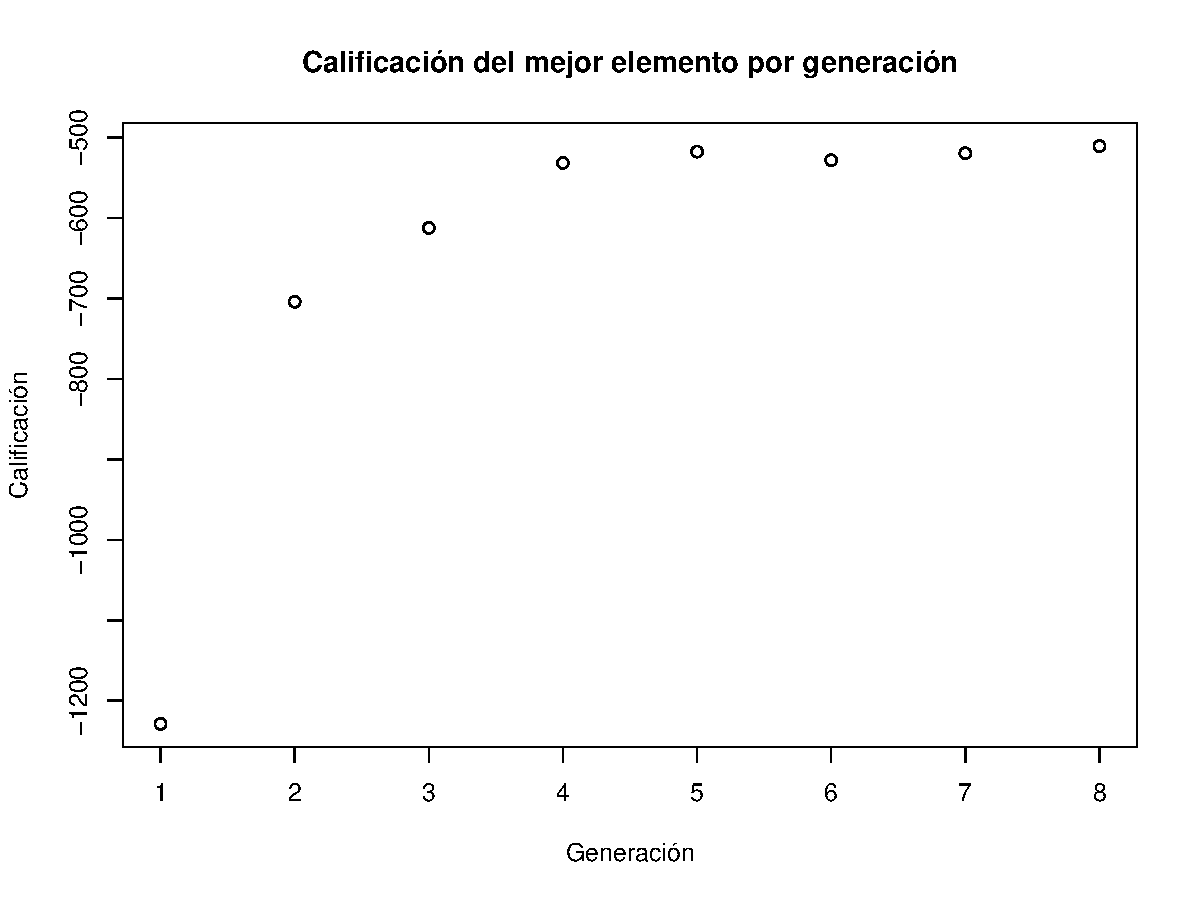
\includegraphics[scale = 0.7]{calif_mejores_hijos_g08_n08_m004_U510.pdf} %width=\textwidth
%\caption[\textit{Calificaciones de las mejores asignaciones por generación}]{\textit{Se muestran las calificaciones de la mejor asignación por generación. Se observa una mejora considerable en la calificación de la generación 1 a la 2.}}\label{EjcalifMejoresHijos}
%\end{figure}

En la \figurename{~\ref{boxplot_calif_x_generacion}} observamos las gráficas de caja de las calificaciones de las asignaciones, para cada generación. Hay una mejora considerable en las calificaciones de la generación 1 a la 2. Los puntos representan las calificaciones de cada asignación por generación. Notamos que las calificaciones de las asignaciones en la generación 6, son muy parecidas. A diferencia de las calificaciones en la generación 3, las cuales varían más.

%\begin{figure}[H]
%\centering
%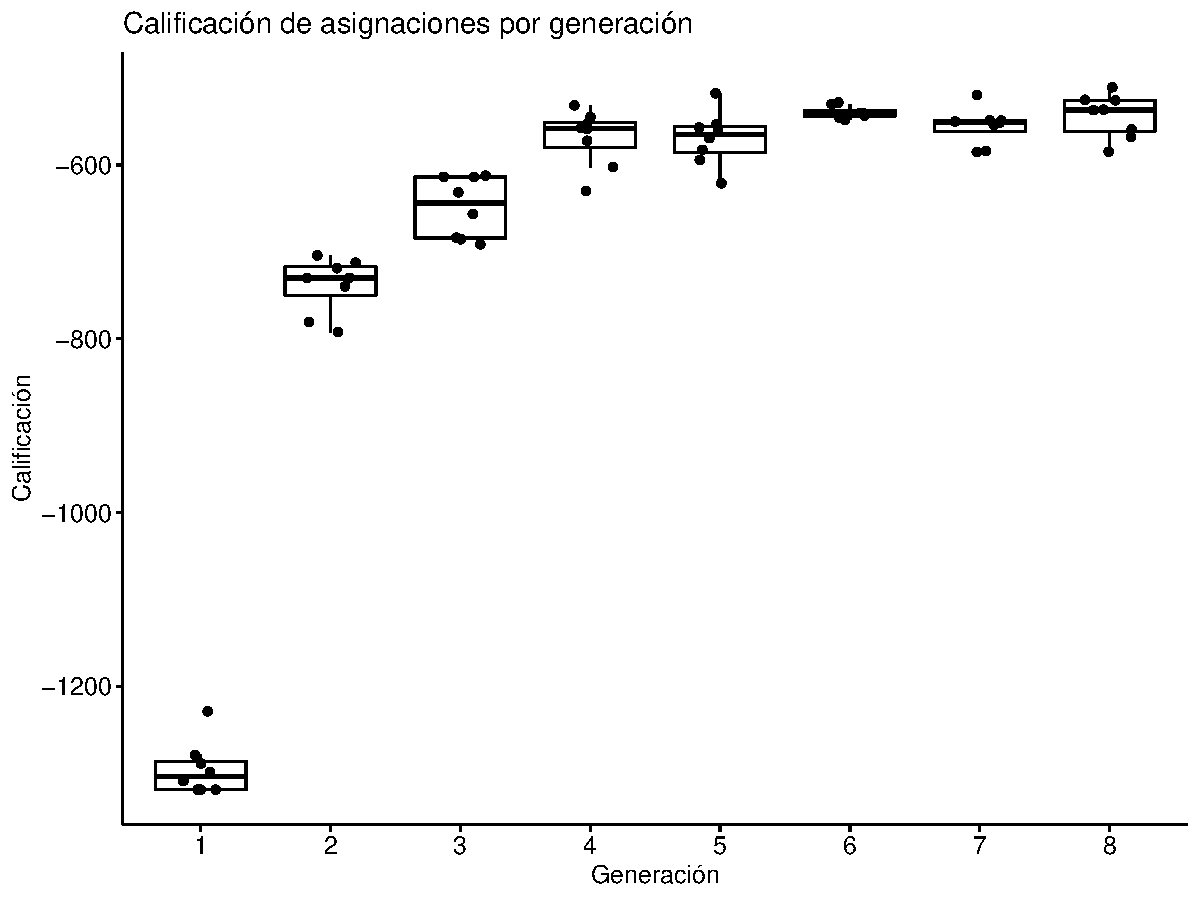
\includegraphics[scale = 0.7]{boxplot_calif_g08_n08_m004_U510.pdf} %width=\textwidth
%\caption[\textit{Gráficas de caja de calificaciones de asignaciones por generación}]{\textit{Se muestran las gráficas de caja de las calificaciones de las asignaciones por generación. Se observa una mejora considerable en la calificación de la generación 1 a la 2.}}\label{boxplot_calif_x_generacion}
%\end{figure}

En la \figurename{~\ref{media_calif_x_generacion}} se puede ver el promedio de las calificaciones de las asignaciones por generación. Al igual que en las Figuras \ref{EjcalifMejoresHijos} y \ref{boxplot_calif_x_generacion} se observa una mejora considerable en la calificación de la generación 1 a la 2. Podemos observar que el promedio de las calificaciones de la generación 7 es menor que el promedio de las calificaciones de la generación 6.


%\begin{figure}[H]
%\centering
%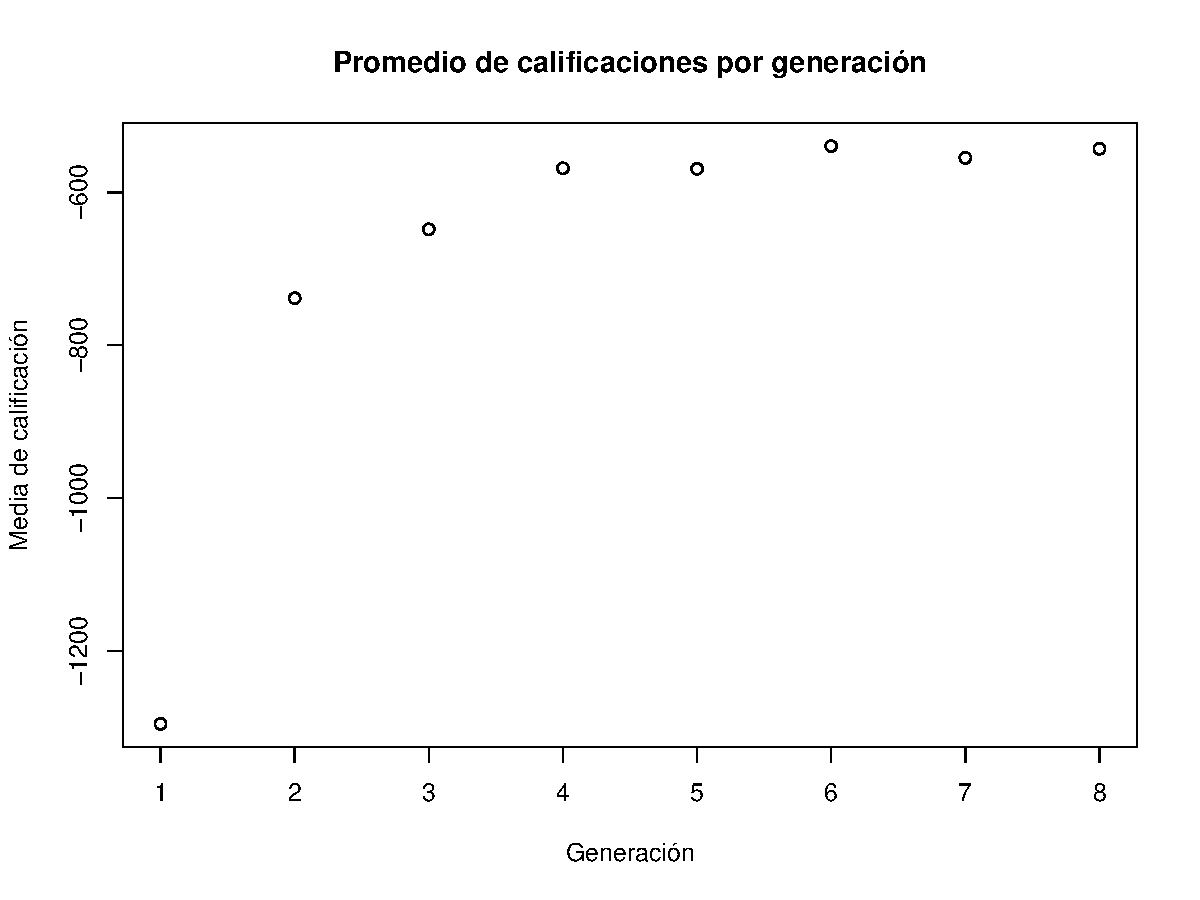
\includegraphics[scale = 0.7]{media_calif_g08_n08_m004_U510.pdf} %width=\textwidth
%\caption[\textit{Media de calificaciones de asignaciones por generación}]{\textit{Se muestra el promedio de las calificaciones de las asignaciones por generación. Se observa una mejora considerable en la calificación de la generación 1 a la 2.}}\label{media_calif_x_generacion}
%\end{figure}

En la \figurename{~\ref{var_calif_x_generacion}} se ve la varianza de las calificaciones de las asignaciones por generación. El valor más pequeño se observa en la generación 6. Al ver la \figurename{~\ref{boxplot_calif_x_generacion}} en dicha generación, notamos que los puntos tienen valores muy similares. La varianza más grande se obtiene en la generación 3. Ésto también se puede ver en la \figurename{~\ref{boxplot_calif_x_generacion}}.


\begin{figure}[H]
\centering
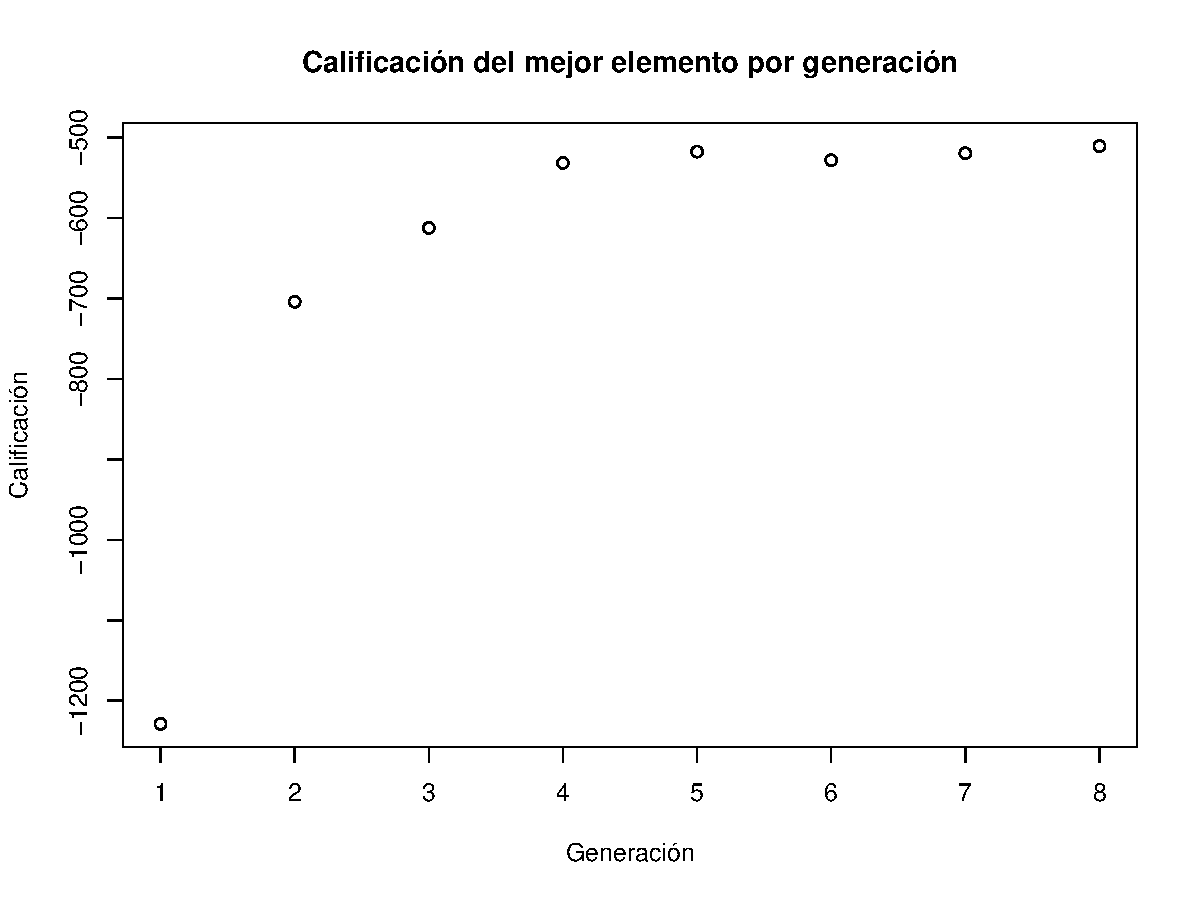
\includegraphics[scale = 0.67]{calif_mejores_hijos_g08_n08_m004_U510.pdf} %width=\textwidth
\caption[\textit{Calificaciones de las mejores asignaciones por generación}]{\textit{Se muestran las calificaciones de la mejor asignación por generación. Se observa una mejora considerable en la calificación de la generación 1 a la 2.}}\label{EjcalifMejoresHijos}
\end{figure}


\begin{figure}[H]
\centering
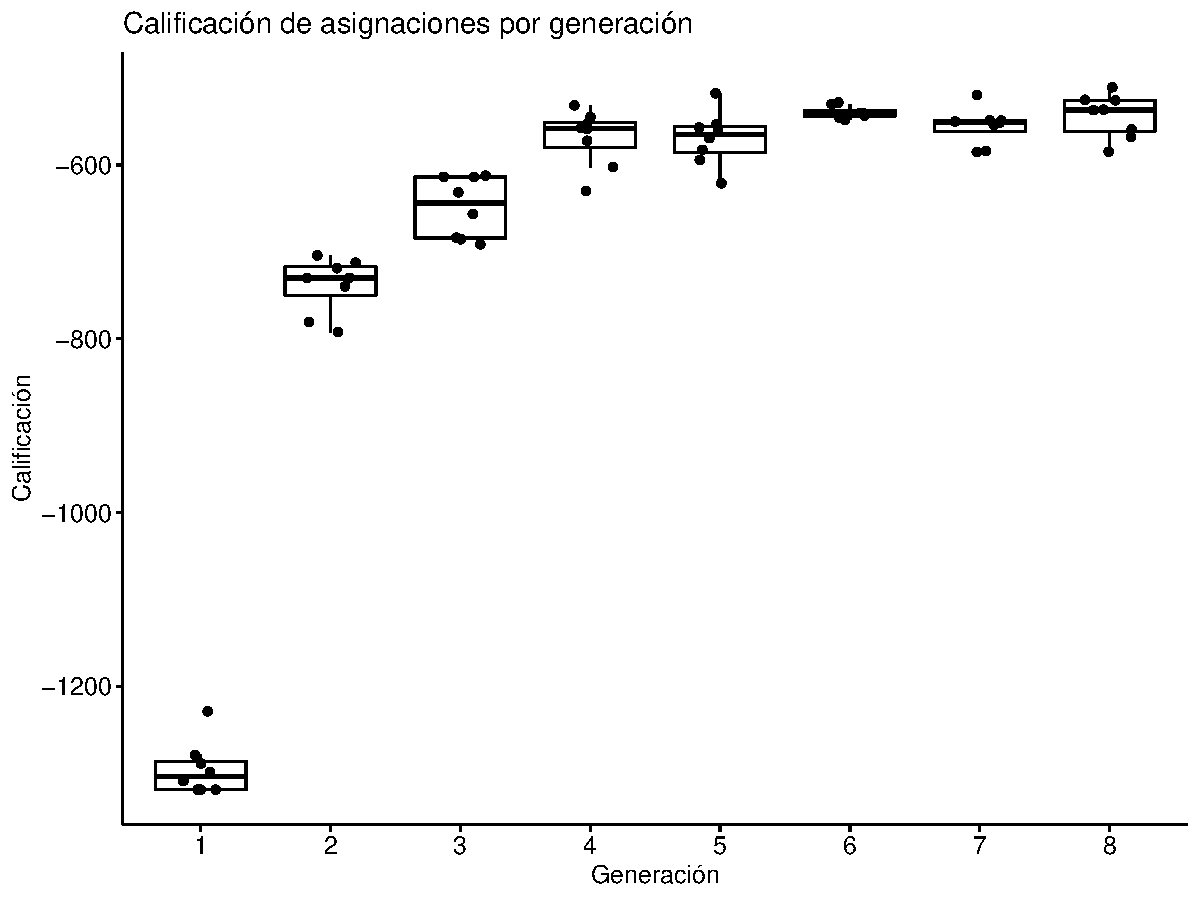
\includegraphics[scale = 0.67]{boxplot_calif_g08_n08_m004_U510.pdf} %width=\textwidth
\caption[\textit{Gráficas de caja de calificaciones de asignaciones por generación}]{\textit{Se muestran las gráficas de caja de las calificaciones de las asignaciones por generación. Se observa una mejora considerable en la calificación de la generación 1 a la 2.}}\label{boxplot_calif_x_generacion}
\end{figure}

\begin{figure}[H]
\centering
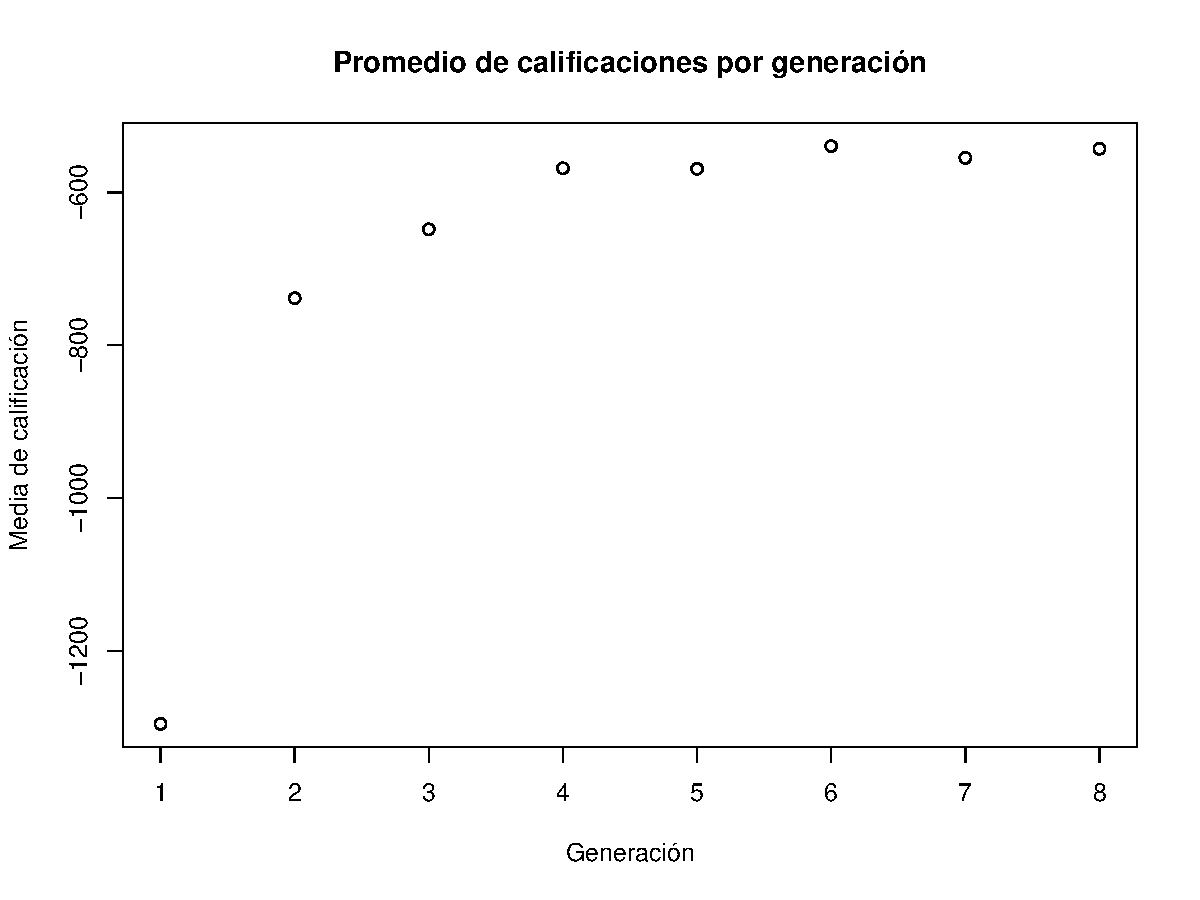
\includegraphics[scale = 0.67]{media_calif_g08_n08_m004_U510.pdf} %width=\textwidth
\caption[\textit{Media de calificaciones de asignaciones por generación}]{\textit{Se muestra el promedio de las calificaciones de las asignaciones por generación. Se observa una mejora considerable en la calificación de la generación 1 a la 2.}}\label{media_calif_x_generacion}
\end{figure}


\begin{figure}[H]
\centering
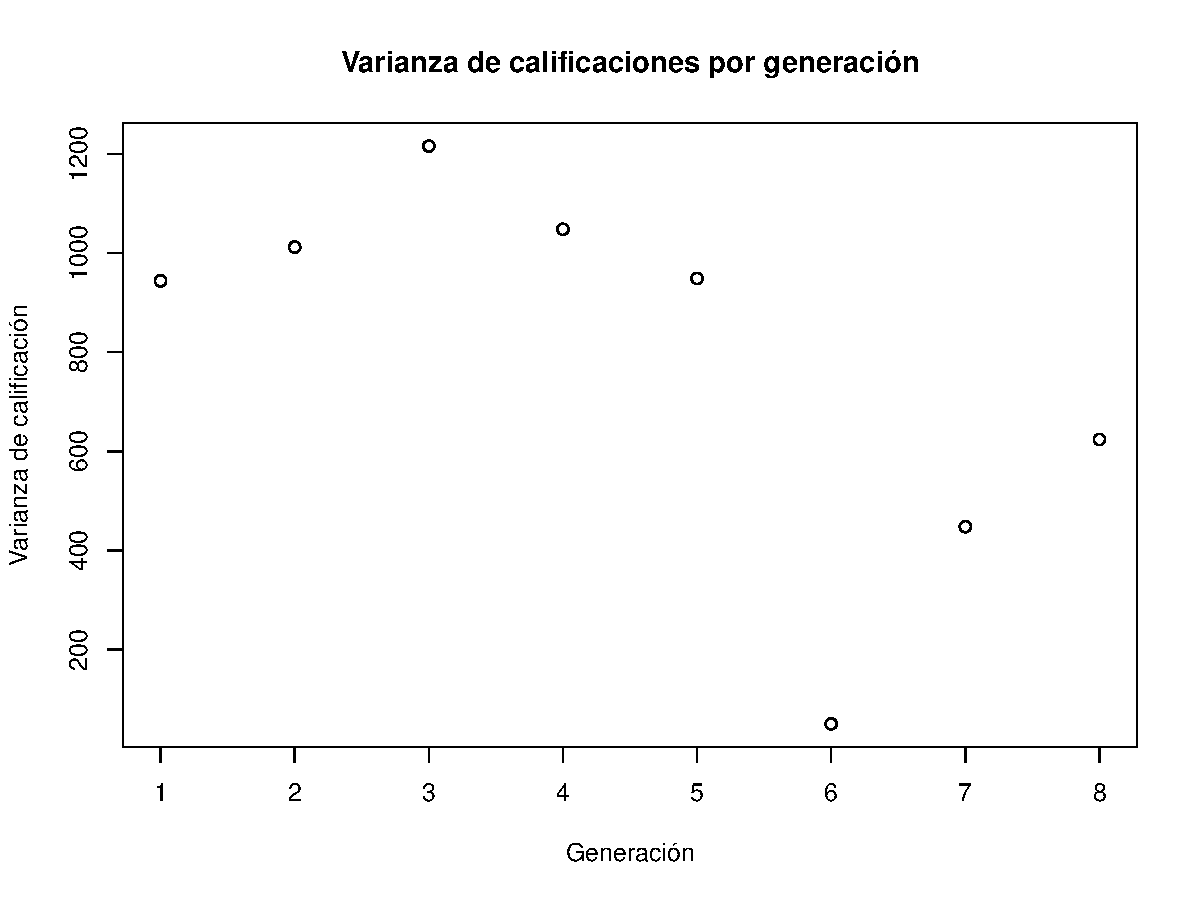
\includegraphics[scale = 0.67]{varianza_g08_n08_m004_U510.pdf} %width=\textwidth
\caption[\textit{Varianza de calificaciones de asignaciones por generación}]{\textit{Se muestra la varianza de las calificaciones de las asignaciones por generación. Se observa una disminución considerable de la generación 5 a la 6. El valor más grande se encuentra en la generación 3.}}\label{var_calif_x_generacion}
\end{figure}

En la \figurename{~\ref{boxplot_num_genes_x_generacion}} podemos ver las gráficas de caja del número de genes en las asignaciones por generación. Los puntos representan el número de genes de cada asignación por generación. Notamos que la media de la generación 2 es considerablemente mayor que la media de la generación 1.

De la generación 1 a la 6 los promedios del número de genes tienden a ser cada vez mayores. Ésto se logra al agregar los grupos que aún se pueden asignar después de hacer el cruce con los padres.

También podemos observar que el promedio del número de genes en las generaciones 7 y 8 es menor al promedio del número de genes en la generación 6. En las generaciones 4 y 7, el número de genes varía mucho.

\begin{figure}[h]
\centering
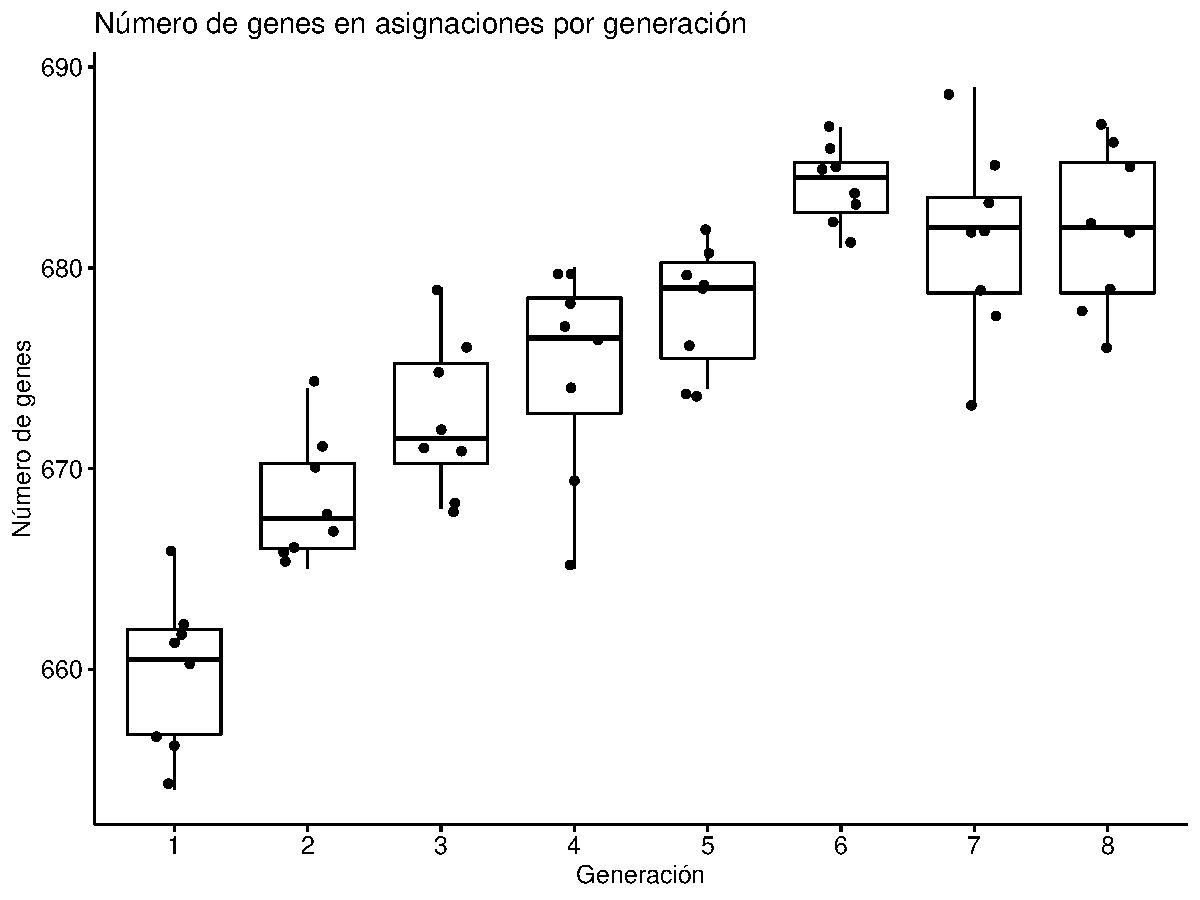
\includegraphics[scale = 0.7]{boxplot_num_genes_g08_n08_m004_U510.pdf} %width=\textwidth
\caption[\textit{Gráficas de caja del número de genes en asignaciones por generación}]{\textit{Se muestran las gráficas de caja del número de genes en asignaciones por generación. Se observa que los valores tienen una tendencia no decreciente.}}\label{boxplot_num_genes_x_generacion}
\end{figure}

%****************************************************************************

%En un esqueleto simulado para el 2020-2 se tuvieron 1018 grupos. De éstos se asignaron 612. Encontramos que 262 grupos sin asignación correspondían a materias optativas. Prácticamente $\dfrac{1}{4}$ de los grupos no asignados son de materias optativas. Ésto se debe a que se pueden asignar \textit{num\_max\_asig} materias obligatorias a los profesores por lo que ya no se les asignan las optativas. En la matriz de solicitudes puede haber grupos que no están en la asignación final. Ésto por el cruce de los padres.
%
%\begin{eqnarray*}
%\dfrac{612}{1018} &=& 60.11\% \text{grupos asignados}\\
%\dfrac{262}{1018} &=& 25.73\% \text{grupos de optativas sin asignación}\\
%\dfrac{1018 - (612 + 262)}{1018} &=& \dfrac{144}{1018} = 14.14\% \text{grupos de obligatorias sin asignación}
%\end{eqnarray*}

%\begin{figure}[H]
%\centering
%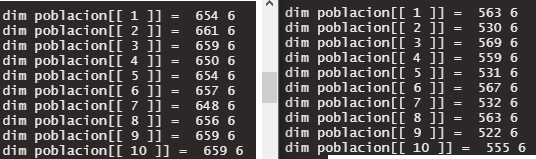
\includegraphics[width=\textwidth]{num_genes_generaciones_1_2} %scale = 0.7
%\caption[\textit{Número de genes en generaciones 1 y 2}]{\textit{Número de genes en generaciones 1 y 2}}
%\end{figure}

%Sabemos que la asignación final es el mejor elemento de la última generación. En la \tablename{~\ref{submatAsigFinal}} presentamos una submatriz de la asignación final. Cabe aclarar que los datos se ordenaron con respecto a la materia (en orden alfabético) y por hora (de menor a mayor). La matriz completa se puede ver el el Apéndice \ref{Ej_AsigFinal}. Dicha matriz tiene 630 grupos asignados, cada uno con materia, profesor y horario correspondiente. En el semestre 2020-1 se tuvieron 747 grupos reales. Se simularon 1011 grupos en \textit{mat\_esqueleto}. Las materias optativas y obligatorias de los siguientes porcentajes se consideran con respecto a la carrera de Actuaría.
%
%\begin{eqnarray*}
%\dfrac{630}{1011} &=& 62.31\% \text{grupos asignados}\\
%\dfrac{229}{1011} &=& 22.65\% \text{grupos de optativas sin asignación}\\
%\dfrac{17}{1011} &=& 1.68\% \text{grupos de inglés sin asignación}\\
%\dfrac{1011 - (630 + 229 + 17)}{1011} &=& \dfrac{135}{1011} = 13.35\% \text{grupos de obligatorias sin asignación}\\
%\dfrac{630}{747} &=& 84.33\% \text{grupos asignados comparado con el 2020-1}
%\end{eqnarray*}

Sabemos que la asignación final es el mejor elemento de la última generación. En la \tablename{~\ref{submatAsigFinal}} presentamos una submatriz de una asignación final. Cabe aclarar que los datos se ordenaron con respecto a la materia (en orden alfabético) y por hora (de menor a mayor). La matriz completa se puede ver en el Apéndice \ref{Ej_AsigFinal}.

Dicha matriz tiene 682 grupos asignados, cada uno con materia, profesor y horario correspondiente. En el semestre 2020-1 se tuvieron 747 grupos reales. Se simularon 1091 grupos en \textit{mat\_esqueleto} para el semestre 2020-2.

\begin{table}[H]
\centering
\begin{tabular}{|c|p{7cm}|p{4.7cm}|c|}
\hline
\textbf{ } & \textbf{Materia} & \textbf{Profesor} & \textbf{Horario} \\ \hline
1 & Administración Actuarial del Riesgo & Fernando Pérez Márquez & 7 \\ \hline
  133 & Cálculo Diferencial e Integral I & Elena de Oteyza de Oteyza & 7 \\ \hline
  156 & Cálculo Diferencial e Integral II & Héctor Méndez Lango & 11 \\ \hline
%  353 & Inferencia Estadística & Martha Angélica Montes Fonseca & 18 \\ \hline
  401 & Manejo de Datos & José Alfredo Cobián Campos & 13 \\ \hline
  418 & Matemáticas Financieras & Irma Rocío Zavala Sierra & 7 \\ \hline
  498 & Modelos de Supervivencia y de Series de Tiempo & Margarita Elvira Chávez Cano & 10 \\ \hline
%  505 & Modelos no Paramétricos y de Regresión & Jaime Vázquez Alamilla & 8 \\ \hline
  510 & Modelos no Paramétricos y de Regresión & Lizbeth Naranjo Albarrán & 11 \\ \hline
  534 & Probabilidad I & María Asunción Begoña Fernández Fernández & 10 \\ \hline
  539 & Probabilidad II & Daniel Alejandro Zurita Gutiérrez & 8 \\ \hline
  561 & Procesos Estocásticos I & Arrigo Coen Coria & 10 \\ \hline
  567 & Productos Financieros Derivados & Jesús Agustín Cano Garcés & 10 \\ \hline
%  679 & Variable Compleja I & Micho Durdevich Lucic & 16 \\ \hline
%  680 & Variable Compleja I & Mico Djurdjevic & 16 \\ \hline
  682 & Variable Compleja I & Jesús Manuel Mayorquín García & 19 \\ \hline
\end{tabular}
\caption[\textit{Submatriz con asignación final}]{\textit{Se muestra una submatriz de la asignación final. Cada renglón tiene la información de un grupo con una materia, profesor y horario asignado.}}\label{submatAsigFinal}
\end{table}


A continuación presentamos algunos porcentajes que nos permiten hacer diferentes comparaciones. Las materias optativas y obligatorias que se mecionan, se consideran con respecto a la carrera de Actuaría.

\begin{eqnarray*}
\dfrac{682}{1091} &=& 62.51\% \text{ grupos asignados}\\\\
\dfrac{409}{1091} &=& 37.48\% \text{ grupos no asignados}\\\\
\dfrac{241 + 18}{1091} &=& 23.73\% \text{ grupos de optativas e inglés sin asignación}\\\\
%\dfrac{18}{1091} &=& 1.64\% \text{ grupos de inglés sin asignación}\\\\
\dfrac{150}{1091} &=& 13.74\% \text{ grupos de obligatorias sin asignación}\\\\ %\dfrac{1091 - (682 + 241 + 18)}{1091}
\dfrac{682}{747} &=& 91.29\% \text{ grupos asignados comparados con el 2020-1}
%\dfrac{1091}{747} &=& 146.05\% \text{ grupos simulados para 2020-2 comparados con el 2020-1}
\end{eqnarray*}

%\begin{figure}[H]
%\centering
%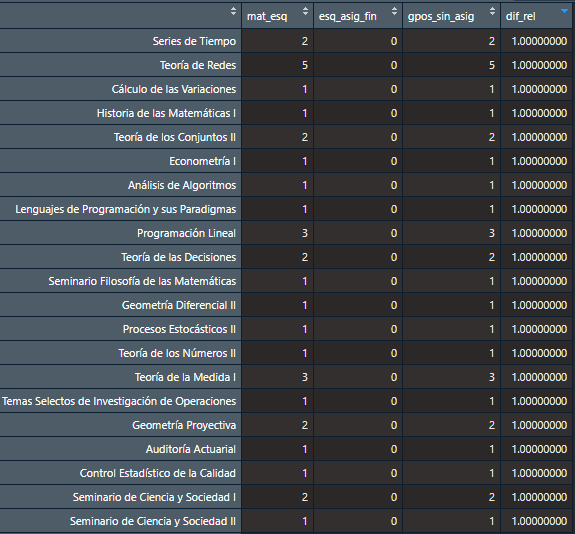
\includegraphics[width=\textwidth]{dif_rel_optativas_sin_gpo} %scale = 0.7
%\caption[\textit{Optativas sin grupos asignados}]{\textit{Optativas sin grupos asignados}}
%\end{figure}

Notamos que casi una cuarta parte de los grupos simulados en \textit{mat\_esqueleto} corresponde a materias optativas y de inglés sin asignación. Ésto ocurre por dos principales motivos:

\begin{enumerate}
\item No hay solicitudes en \textit{mat\_solicitudes} de los grupos no asignados. Existen materias optativas que no se imparten todos los semestres. Por ello hay ocasiones en las que no se simula la solicitud.

\item Se les asigna otra materia a esa hora a los profesores que hayan solicitado alguna optativa. Usualmente se les asigna una obligatoria a la hora en la que solicitaron la optativa.
\end{enumerate}

La principal razón por la que se tiene alrededor de un $10\%$ de materias obligatorias sin asignar es por la forma en la que definimos \textit{mat\_esqueleto}. El modelo de mezcla de normales nos permite que los grupos se distribuyan a lo largo de las horas sin tener picos demasiado altos.

Ésto se basa en el supuesto de que los alumnos tienen la misma preferencia por una materia a cierta hora, o a la hora anterior o a la siguiente. Es decir, si un alumno elige \textit{Probabilidad I} a las 10hrs, le es indistinto si la toma a las 9hrs, a las 10hrs o a las 11hrs.

Este fenómeno se observa con mayor claridad en las materias con horarios muy específicos como \textit{Teoría del Seguro, Matemáticas Actuariales para Seguro de Daños, Fianzas y Reaseguro} o \textit{Matemáticas Actuariales del Seguro de Personas I}.

En el caso de \textit{Teoría del Seguro} se simularon 4 grupos en \textit{mat\_esqueleto}, a las 8hrs, 10hrs, 13hrs y 19hrs. Las solicitudes simuladas se pueden ver en la \figurename{~\ref{sol_TeoSeguro}}. Notamos que sólo hay solicitudes a las 8hrs y a las 19hrs. Con estos datos el algoritmo sólo puede asignar dos grupos, uno a las 8hrs y otro a las 19hrs.

\begin{figure}[H]
\centering
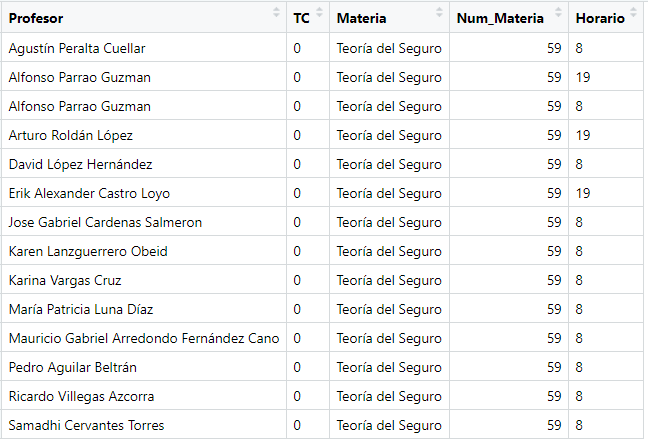
\includegraphics[scale = 0.8]{solicitudes_teoria_del_seguro} %width=\textwidth
\caption[\textit{Solicitudes simuladas de la materia ``Teoría del Seguro'' para el semestre 2020-2}]{\textit{Se muestran las solicitudes simuladas de la materia ``Teoría del Seguro'' para el semestre 2020-2.}}\label{sol_TeoSeguro}
\end{figure}

Por estas razones el algoritmo asigna alrededor del $60\%$ de los grupos simulados. Para aumentar este porcentaje, se pueden definir manualmente grupos de materias optativas o de inglés. Ésto en el archivo de excel definido en el paso \ref{paso_cero} del algoritmo. Dado que se elimina la información en las solicitudes antes de realizar el AG, no se tienen grupos repetidos en la asignación final.

